%\chapter{From Tools to Assistants: Real-World Applications}\label{sec:assist}
\chapter[From Tools to Assistants]{From Tools to Assistants: Real-World Applications}
\label{sec:assist}

\begin{learningbox}
In this chapter you will learn how agentic language models are 
deployed as practical assistants across real-world domains. 
Specifically, you will be able to:
\begin{itemize}[leftmargin=*, nosep]
    \item Describe how assistants go beyond question answering to plan, retrieve information, invoke tools, and {\em adapt their behavior} over time.
    \item Compare assistant architectures across  domains including {\em shopping, medicine, aviation, scientific research and  coding}
    .
    \item Explain why high-risk domains impose stricter requirements  around {\em safety, transparency, and regulatory compliance} and how agentic designs respond to these demands.
    \item Critically evaluate assistant behavior and reflect on the  {\em ethical} implications of deploying agentic systems in socially consequential settings.
\end{itemize}
\end{learningbox}

\section{Agentic LLMs as Assistants}
LLMs have moved from text generators to active assistants.  
They combine reasoning, retrieval, and tool use to perform actions in the real world.  
Assistants are the practical (software) form of agentic LLMs: systems that interact, plan, and learn from feedback. 
Assistants are where reasoning meets reality:  
they turn language models into collaborative actors in the world.

An assistant links perception, reasoning, and action.  
Through APIs and external tools, it can converse, execute tasks, and adapt to a specific context. These systems not only support users but also create valuable human-AI interaction data that we can then use for further developments and training the next generation of models.

This chapter reviews the main types of assistants.  
We start with conversational systems and their evolution toward multi-modal, tool-aware interfaces.  
Next, we discuss domain-specific assistants in medicine, finance, and trading.  
Finally, we look at scientific assistants for reasoning and discovery.


%\chapter{Assistants}
% \section{Conversation}

% The progress in reasoning and decision making has improved the accuracy and usability of LLMs for
% everyday tasks. Also, LLMs can act through their use of
% tools. Tool-enabled LLMs can  be used as virtual assistants. There is commercial interest in this 
% element of Agentic AI, and much activity has been reported.
% %
% Furthermore, assisting humans generates more training data, on which LLMs can be pretrained and finetuned.

% We start our review with conversational assistants, and then continue to
% shopping, travel, medical, and financial trading support.

\section{Conversational  Assistants}

The first application domain is in general conversational situations, such as helping with meetings by taking  meeting minutes, acting as meeting chair or general administrative assistant.

In this type of application, the LLM basically serves to make the interaction between human and computer more natural and streamlined \citep{neszlenyi2024assistantgpt,oluwagbade2024conversational}. For example, the AssistantGPT system \citep{neszlenyi2024assistantgpt} is a  general purpose administrative assistant, designed for deployment in an educational or corporate
setting. Furthermore, it  supports remote work environments such as Teams and Slack. AssistantGPT supports a diverse range of operations, including web searches, API interactions via OpenAPI, voice conversations, and command execution through the shell. The system consists of an LLM with access to various tools such as a planner, and memory (see Figure~\ref{fig:assist}). 

\begin{figure}
  \begin{center}
    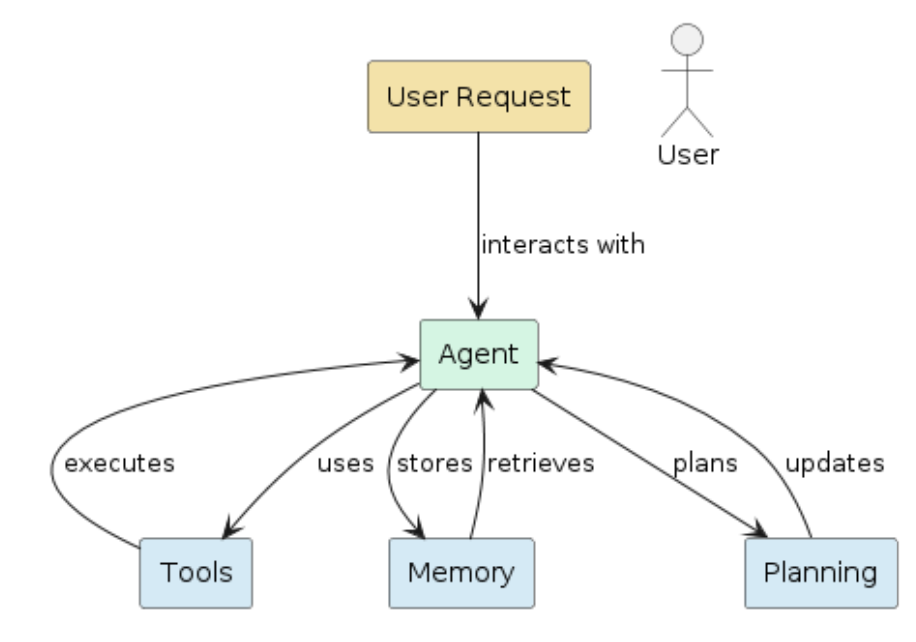
\includegraphics[width=9cm]{figures/assist}
    \caption{AssistGPT system architecture  \citep{neszlenyi2024assistantgpt}}\label{fig:assist}
  \end{center}
\end{figure}

These conversation and meeting assistants have been shown to 
improve agile software development team meetings \citep{cabrero2024exploring}. They created favorable results for preparation  and live assistance during Scrum meetings, although some testers remarked that LLM interventions felt
unnatural and inflexible. %Marking some early results and limitations of LLMs as conversational agents.

Other examples include LLM agents in a collaborative learning classroom setting where the LLM agents improved overall collaboration between participants \citep{wei2024improving}. Another study \citep{bastola2023llm} reports improved work efficiency in a collaborative task scheduling experiment including conversational assistants.  

A slightly different type of assistant is the thinking assistant. This assistant tries to improve human reflective thinking for difficult decisions,  by asking instead of
answering \citep{park2023thinking}.  Similar initiatives have recently appeared from the large LLM vendors, such as {\em Study mode} in OpenAI's ChatGPT and Google's Gemini applications.

Conversational assistants have mostly evolved from regular pretrained LLMs, sometimes finetuned for a particular domain. Some approaches use a specialized multi-LLMs approach,
specializing LLMs for different sub-tasks, or orchestrating a single LLM with different prompt sequences focusing on different sub-tasks.


\section{Shopping Assistant}

In this section we examine how language-based assistants can be applied in the e-commerce domain. Our goal is to highlight the principal components, architectural choices and domain-specific challenges in this domain.

\paragraph{What does a shopping assistant do?}
A shopping assistant is a conversational system built on an LLM that helps users navigate online shopping tasks. It can help in understanding product needs, comparing alternatives, recommending items and completing purchases. Such a system typically complements the underlying LLM with domain-specific modules, including retrieval of up-to-date product information, API access to product-catalogs, integration with recommender engines and reasoning (e.g., via chain of thought) over user requirements, attributes and constraints.

\paragraph{Key ingredients}
Because general-purpose LLMs lack built-in awareness of e-commerce concepts (brands, categories, product hierarchies, user purchase behavior), building a capable assistant requires several augmentations:
\begin{itemize}
  \item Retrieval Augmentation: dynamically fetch product metadata, pricing, availability from external sources.
  \item Tool / API Invocation: the assistant may call search, filter, ranking tools to interact with product databases.
  \item Domain Finetuning or Instruction Tuning: adapt the LLM to the shopping context (branded language, attribute reasoning, user intents).
  \item Structured Reasoning: add chain of thought prompting or explicit reasoning steps. This helps the model compare products, evaluate trade-offs (e.g., price vs features) and align with user preferences.
\end{itemize}

\paragraph{Benchmarking shopping-assistants}
To study how well models cope with shopping-specific tasks, researchers have developed benchmarks. For example, the \emph{Multi-task Online Shopping Benchmark dataset (ShopMMLU)}~\citep{jin2024shopping}  defines 57 tasks grouped into four skills: concept understanding, knowledge reasoning, user-behavior alignment and multi-linguality. It draws on real-world e-commerce data (Amazon product catalogs, sessions and reviews) and evaluates how well an LLM can handle aspects like brand-model recognition, reasoning about product compatibility, session-based recommendation tasks, and multilingual queries.
Another example is the LLaSA system (large language and E-commerce shopping assistant) \citep{zhang2024llasa} which is trained via an instruction dataset (65,000 samples) dubbed {\em EshopInstruct}. After instruction-tuning on shopping tasks, LLaSA competes on the ShopBench benchmark and achieves strong results, showing that adaptation significantly improves performance in this domain. 

\paragraph{Practical Recommendations}
The following principles are important for building shopping assistants:
\begin{itemize}
  \item A capable assistant merges natural-language understanding and domain reasoning. It should know what {\em noise-canceling headphones under 200 euro with > 20 h battery} means, and be able to translate this into product attributes and user constraints.
  \item Domain-specific data matters: off-the-shelf LLMs work to some degree, but fine-tuning or instruction-tuning on shopping tasks significantly lifts performance. LLaSA \citep{zhang2024llasa} shows this in practice.
  \item Evaluation must reflect the domain. Accuracy in understanding product attributes or generating queries is less relevant than whether the assistant can align with user behavior, handle multi-step sessions and support multilingual users.
  \item Tool and retrieval integration is important. The assistant must act as an interface to product systems, not just as a pure language model. This introduces additional complexity (API design, latency, freshness of data and handling integration errors).
  \item Consider ethics and trust. In shopping, recommendations carry commercial, privacy and bias implications. These issues should be assessed before deploying such a system in production, through questions such as: {\em which brands are shown}, {\em is user history handled correctly}, and {\em how transparent is the reasoning}.
\end{itemize}

\paragraph{Challenges and open questions}
Even with recent progress, shopping assistants face several non-trivial challenges. First, handling long interaction trajectories (browsing, refining queries, switching intents) is still difficult for LLM agents. Second, updating product knowledge in real-time (new models, price changes, availability) remains a major engineering pain-point. Third, explaining and justifying recommendations to users (why this product vs another) is under-explored in LLM-based assistants. Finally, cross-lingual behavior and multilingual product queries increase complexity (shopping contexts span languages and regions).


% \section{Shopping Assistant}

% LLM-based shopping assistants extend general-purpose LLMs by tailoring them to the e-commerce domain. These assistants help users search for, compare, and recommend products through natural language interaction. To improve their performance, models are often \emph{finetuned} on shopping-related data or combined with traditional recommender systems. Common techniques include \emph{retrieval augmentation}, \emph{tool use} (e.g., calling APIs for product databases), and \emph{Chain-of-Thought reasoning} for structured decision making.

% Basic LLMs are not naturally aware of e-commerce concepts such as brands, product hierarchies, or shopping intents. To evaluate and improve these abilities, \citet{jin2024shopping} introduced the \emph{Multi-task Online Shopping Benchmark (ShopMMLU)}. This benchmark defines 57 tasks covering four key skills: (1) concept understanding, (2) knowledge reasoning, (3) user behavior alignment, and (4) multilingual comprehension. Together, these tasks capture the core challenges of building capable shopping assistants.

% Several research projects have focused on improving interaction quality and personalization. For instance, \citet{vedula2024question} proposed a system that generates dynamic follow-up questions for shopping assistants, based on product metadata. This approach helps the assistant gather more precise user preferences. Similarly, \citet{chen2024chatshop} developed \emph{ChatShop}, a benchmark designed to assess information-seeking behaviors of conversational agents in shopping scenarios.


% A recent example of an LLM-based e-commerce system is \emph{LLaSa} (\emph{Large Language Shopping Assistant}) introduced by \citet{zhang2024llasa}. The authors constructed a dataset of 65,000 instruction-based samples covering diverse shopping tasks and trained their model using instruction tuning. The resulting assistant achieved strong results on the \emph{ShopBench} benchmark, demonstrating that combining domain-specific data with instruction tuning can produce specialized and effective shopping assistants.

\section{Flight Operations Assistant}

Language-based assistants are also applied in aviation operations, a domain that extends beyond consumer booking and moves into planning and decision support.

\paragraph{Booking and travel-planning}
One of the simpler applications is a conversational booking assistant, similar to the shopping assistants in the previous section. For example, \citet{manasa2024towards} present a system built on LLaMa 2 with RAG to interactively help users book flights. The assistant is fine-tuned on flight-booking data, and connects to current flight information via retrieval. User testing achieved strong marks for capturing user preferences and guiding the booking process efficiently. 

Notice how this use-case remains relatively shallow in operational complexity. The assistant deals with structured user intents ({\em I want to fly from A to B on date D}), retrieval of up-to-date product data, preference elicitation and generation of responses. It does not (yet) deeply engage with, say, dynamic air-traffic constraints or safety margins.

\paragraph{Operational decision support}
Moving to more demanding settings, LLM-based assistants are  being proposed for actual flight operations. We discuss two examples.

In a study by \citet{zhou2024flight}, the arrival-slot-allocation problem (i.e., determining in which sequence arriving aircraft should land) is formulated as a language modeling task. The authors encode the scheduling inputs and outputs as tokens and fine-tune an LLM to generate conflict-free landing sequences. Their experiments show that the model can reduce conflict rate and total delay time even for airports where traditional methods struggle.

Another operational problem is planning under environmental hazards. \citet{tabrizian2024using} use chain of thought to support routing or flight plan generation under wind-hazard constraints. Here, the assistant’s task is no longer simply {\em book a flight} but it has to reason about constraints (wind, routing, aircraft performance) and propose operationally feasible plans. 

\paragraph{Key recommendations}
These studies illustrate several important aspects of agentic systems with LLMs:

\begin{itemize}
    \item Tool/Backend Integration: in operational assistants, the LLM must not only converse but also interface with flight-databases, weather feeds, routing engines and slot‐allocation systems. This means implementing tool invocation, retrieval pipelines and decision logic.
    \item Reasoning under Constraints: these assistants must handle combinatorial or scheduling constraints, generate plans, and deal with real‐time uncertainties (such as weather, runway availability). The arrival-slot example is a good example, where the LLM must reason about dynamic sequencing.  
    \item Domain-specific Data and Finetuning: the standard pretrained LLM lacks priors about aviation operations. The systems above are finetuned or prompted specifically for the domain. A dataset of domain-tasks, prompts, expected outputs are evaluation metrics tailored to the domain are necessary.
    \item From Conversational Agent to Autonomous Planner: while booking assistants remain user-driven (the user asks, the assistant helps), operational assistants increasingly take on planning roles. The assistant should handle requests such as {\em here are constraints, propose a schedule or route}. This change raises issues of trust, verification and explainability.
    \item Evaluation in Real Contexts: the evaluation of operational systems often involves more than {\em does the assistant answer the user?}, but also measure aspects such as conflict rate, delay time, and sequence efficiency. For example, the arrival-slot LLM study measured total delay and conflict rate.  
\end{itemize}



\section{Medical Assistant}
Medicine is one of the most active application domains for LLM-based assistants \citep{thirunavukarasu2023large,clusmann2023future,mehandru2024evaluating}.
Recent studies report that LLMs can outperform trained physicians on diagnostic tasks
\citep{goh2024large} and exceed human medical scribes in clinical note generation
\citep{yuan2024continued}. Other evaluations confirm these strengths, while also identifying
systematic weaknesses in specific clinical scenarios \citep{panagoulias2024evaluating}.

Agentic architectures are increasingly used to address regulatory, ethical, and usability
requirements. \citet{sudarshan2024agentic} present an agentic workflow for generating
patient-friendly medical reports that comply with the 21st Century Cures Act. Their system
uses reflexion (Section~\ref{sec:self-reflection}, \citep{shinn2024reflexion}) to iteratively improve clarity and correctness before information is released to patients.

Other studies explore the use of LLM agents for broader clinical support. \citet{qiu2024llm} identify
applications ranging from clinical workflow automation to multi-agent diagnostic support, although  concerns remain regarding accuracy, completeness, and hallucinations.
A scoping review by \citet{ullah2024challenges} emphasizes that medical domain knowledge and ethical constraints are essential when training and fine-tuning such systems.

To mitigate common failure modes, \citet{das2024improved} propose an agentic retrieval-based architecture in which the LLM acts as a planner rather than a direct answer generator. The agent coordinates specialized tools to retrieve and synthesize evidence from trusted medical
sources, reducing hallucinations and \emph{lost-in-the-middle} errors.

\paragraph{High-risk application domain}
Medicine is a high-risk application domain, where incorrect or biased outputs can have direct consequences for patient safety. As a result, medical AI systems are subject to strict regulatory frameworks, including the EU AI Act, which classifies many medical uses of AI as high-risk. Transparency, fairness, and accountability therefore play a central role, both in clinical practice and in academic research on medical LLMs. 
These concerns motivate increased interest in methods that go beyond post-hoc explanations and aim to understand model behavior at a deeper level. We return to this topic in the chapter on \emph{mechanistic interpretability} (Chapter \ref{chap:mi}), where techniques for analyzing and controlling internal model representations are discussed.

\paragraph{Medical education}
In medical education, agentic systems are used to simulate realistic training environments.
\citet{wei2024medco} introduce a multi-agent copilot that supports case-based learning and clinical reasoning practice (Figure~\ref{fig:medco}). For systematic evaluation of medical retrieval-augmented generation, a dedicated benchmark is provided by
\citet{qiao2024benchmarking}.

%
\begin{figure}
  \begin{center}
    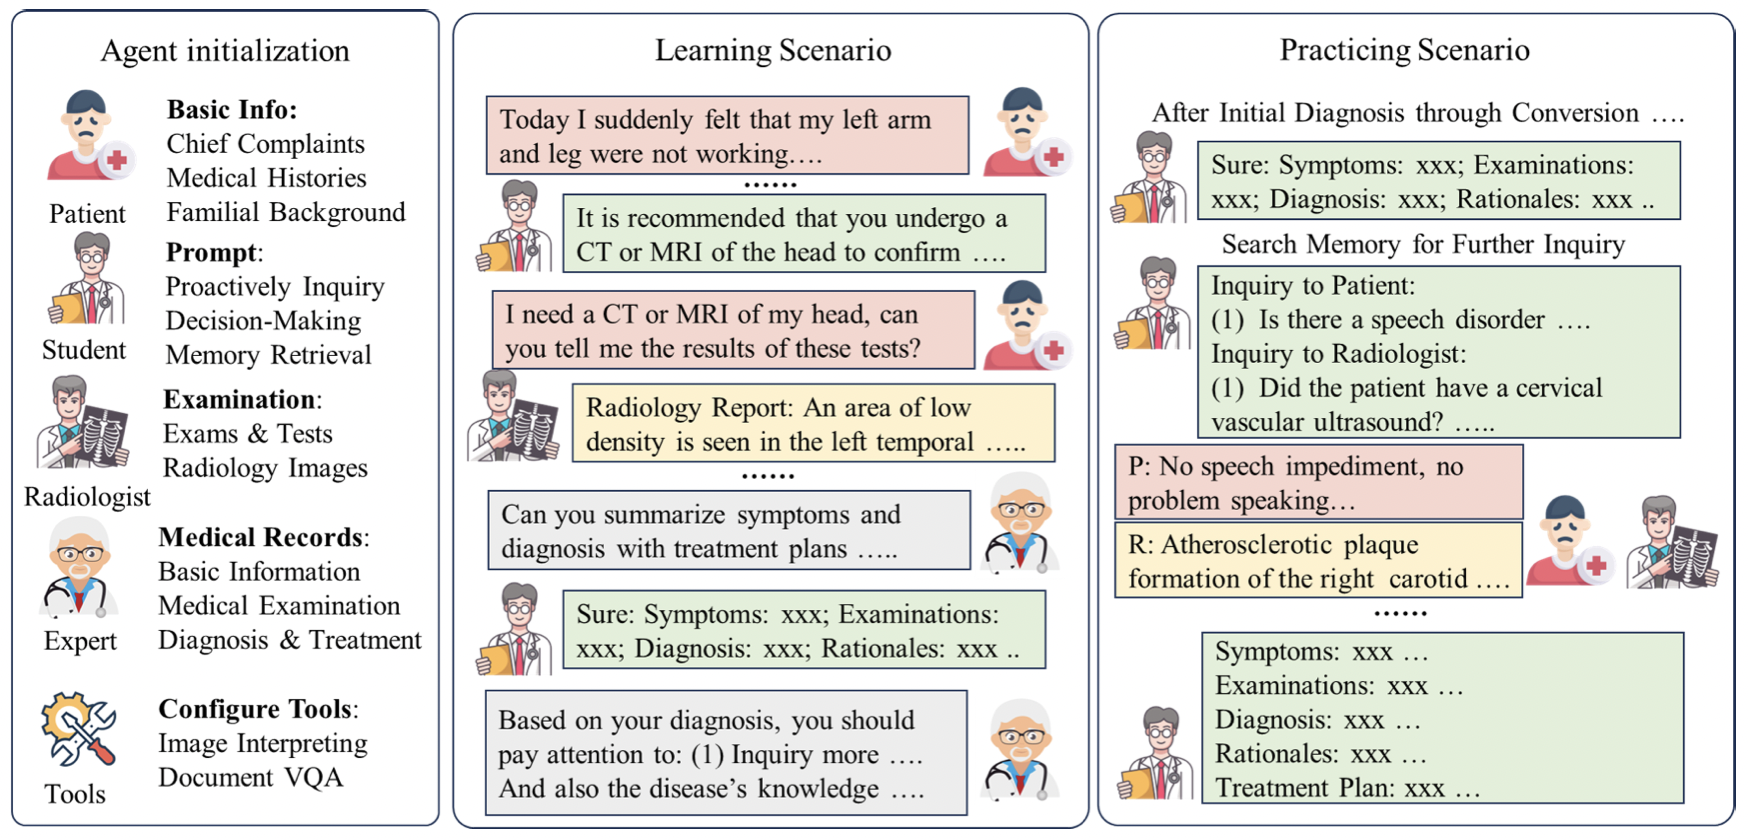
\includegraphics[width=\linewidth]{figures/medco}
    \caption{Medical Education Copilot  \citep{wei2024medco}}\label{fig:medco}
  \end{center}
\end{figure}
%
%A benchmark for retrieval-augmented generation in the medical domain is \citet{qiao2024benchmarking}.

% \subsubsection{Legal Assistant}
% Other domains are also exploring LLMs. The legal domain has much structured, textual, information and
% recently interest in  language models for the legal sector has arisen \citep{padiu2024extent}. 

% Two benchmarks for performance of LLM in the legal domain are
% \citet{guha2022legalbench,li2024legalagentbench}. LegalBench
% contains 44 tasks that span 4 areas of US law. LegalAgentBench contains
% 300 annotated tasks in the Chinese legal domain. 

% % \citet{zhuge2024agent} introduces the Agent-as-a-Judge framework
% % Software development


% % \citep{wu2023precedent} LLM, but No agent
% \citet{buchicchio2024design} describe the architecture of a system
% designed to support legal experts in the process of generating
% summaries from judgments. Nice, but no agent.

% Education: \cite{nelson2024other}



\section{Trading Assistant}
% Can they help financial trading?
A further specialized domain is financial trading. 
Already many (non-LLM) algorithms are used
in financial organizations for trading decisions. The interest in
agentic LLMs in the financial world is large \citep{ding2024large}.

InvestorBench is a benchmark for financial trading systems \citep{li2024investorbench}.
%
FinAgent is a tool-augmented multimodal agent  for financial trading
\citep{zhang2024finagent}.
It contains a market intelligence module, which is able to
extract  insights from multi-modal datasets of
asset prices, visual representations, news and expert
analyses. The system can also perform query retrieval and performs
reflection in a low-level module for technical analysis
and in a high-level module to analyze past trading decisions.

FinRobot is an agentic LLM for financial analysis, to assist human traders.
\citep{yang2024finrobot}. FinRobot can provide document analysis and
generation and market forecasts for
individual stocks.
%
FinMem is an agentic LLM  framework devised for financial decision-making
\citep{yu2024finmem}. It features a layered memory system and
adjustable character design for the trading agent. FinMem is inspired
by the generative agents framework by \citet{park2023generative} (see Section~\ref{sec:gen-agent} and Case Study 4).

So far, most financial market machine learning has focused on single agent
systems. An approach called {\em TradingAgents} uses a multi agent
system to replicate real-world trading firms’ collaborative dynamics
\citep{xiao2024tradingagents}. TradingAgents simulates  LLM-powered
agents in specialized roles such as fundamental analysts,
sentiment analysts, technical analysts and traders with varied risk
profiles. The outcome of the system is a  buy or sell
advice to a human manager. A simulation showed that it outperformed baseline models.

\paragraph{Evaluation} Financial trading is a challenging field of research. The competitive interests in financial trading are high, and there is a natural tendency to keep strong research findings private, which creates a tension with the principles of openness and transparency of scientific research. 

Furthermore, despite the abundance of available numerical data in the field, there are relatively few benchmarking studies that compare different agentic LLM  approaches on the same data. A recent benchmarking study found  methodological flaws in some  financial LLM studies, such as selecting short evaluation periods with positive market trends or leakage of test in training data \citep{li2026can}. 
%by integrating agents with distinct roles and risk profiles, including a reflective agent and a  risk  management team, TradingAgents significantly improves trading outcomes compared to baseline models.


% \citep{kar2024agents} hmm

%\citep{easin2024intelligent}
%\Citep{noguer2024evaluating}


% \subsubsection{CrewAI} \url{https://www.crewai.com}


%\subsubsection{Employee}
% Can Agentic LLMs become an employee?
%\citep{devaraju3048architecting}

%\citep{lambert2023measuring}
%\citep{spitale2024appropriateness}

\section{Automated Scientific Discovery}
The workflow of scientific experimentation is relatively standardized in certain fields of science. For example, in machine learning, (1) ideas are generated, (2) a hypothesis is formulated, (3) an experiment is designed, (4) datasets are acquired, (5) experiments are performed, (6) results are interpreted and (7) a report is produced. This standard workflow has attracted researchers to experiment with agentic LLMs for performing scientific research, see \citet{eger2025transforming} for a survey. 

Google and OpenAI have both released Deep Research agents. These agents can perform multi-step research tasks, such as synthesizing online information. They are built with a reasoning LLM and use retrieval augmentation for finding information sources. The systems are able to create  scientific research papers that look impressive, but are often not error-free. 

AI Scientist \citep{lu2024ai} is a framework to automate the process of scientific discovery, from idea generation to paper writing, including a review process. Users must specify a topic and provide an experimentation template and indicate datasets. The authors report experiments in three areas of machine learning: diffusion
modeling, transformer-based language modeling, and learning dynamics, with promising results. To improve idea generation and reviewing, the agent accesses open sources. Current limitations include limited experiments, incorrect implementation if ideas, and visual errors when the paper is produced. On the other hand, rarely are entire results hallucinated.  Nevertheless, results of the AI scientist are recommended to be taken as hints of promising ideas, worthy of a follow up study \citep{lu2024ai}.

Building on top of the AI scientist idea, the Agent Laboratory was proposed \citep{schmidgall2025agent}, an open-source framework that employs specialized LLM-based agents to accelerate the full research cycle. Unlike the AI Scientist, Agent Laboratory is explicitly designed as a co-pilot for human researchers, complementing rather than replacing human ideation.
%
The framework consists of three main phases: \emph{literature review}, \emph{experimentation}, and \emph{report writing}. Each phase is executed by dedicated agents, such as the PhD, Postdoc, and Professor agents, coordinated through a structured pipeline. The system integrates two specialized components: \emph{mle-solver}, responsible for autonomously generating, testing, and refining machine learning code, and \emph{paper-solver}, which produces a complete research report in \LaTeX\ format based on the experimental results. Both solvers employ iterative refinement, self-evaluation, and reward-based scoring to improve code and report quality across cycles.

Evaluation results demonstrate that Agent Laboratory can autonomously generate complete research projects, including executable code and publication-ready reports, at a fraction of the computational cost of comparable systems (approximately \$2.33 per paper using the \texttt{gpt-4o} backend). Human-in-the-loop or co-pilot mode further improves research quality and usability, with participants reporting high satisfaction and continued use intentions. Nonetheless, human oversight remains essential, as automated self-evaluations tend to overestimate research quality compared to human reviewers.

% We can mention sota here

% Overall, Agent Laboratory represents a new class of LLM-based research assistants that move beyond isolated automation toward end-to-end scientific collaboration. By integrating human feedback loops with autonomous planning and experimentation, such systems illustrate how agentic LLMs may evolve into credible partners in scientific discovery—enabling researchers to focus on creativity, interpretation, and innovation rather than on repetitive implementation work.
\section{Coding Assistants and General Advances}

SWE-Agent (short for {\em software engineering agent}) \citep{yang2024swe} aims to automate the process of software discovery, to help agents to autonomously use computers to solve software engineering tasks. SWE-agent introduces tools to create and edit code files, navigate through software repositories, and execute computer programs. Experiments on coding benchmarks such as HumanEvalFix achieve high success rates of over 80\%. This success is attributed to the interactive design of the agent (see Figure~\ref{fig:swe}). 


\begin{figure}
  \begin{center}
    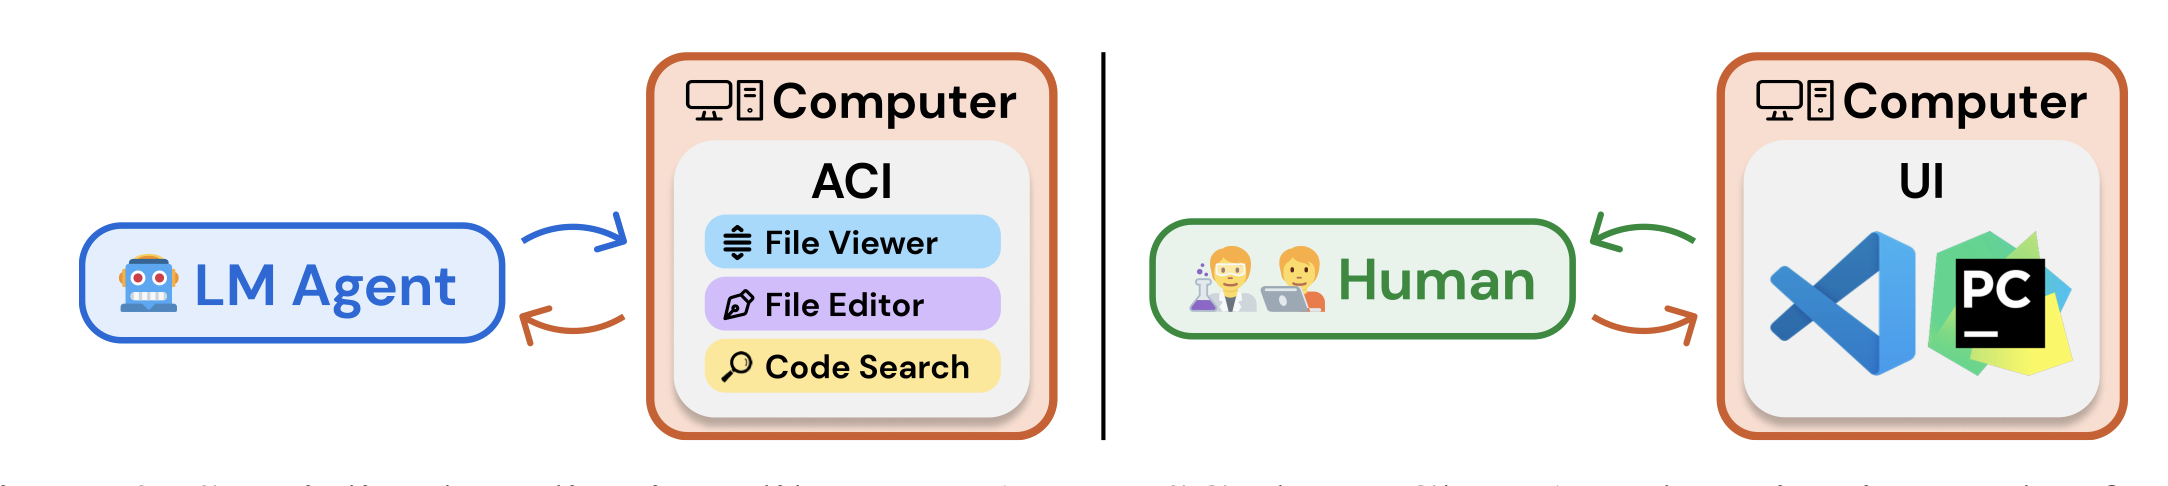
\includegraphics[width=12cm]{figures/swe}
    \caption{SWE-Agent for Software Engineering  \citep{yang2024swe}}\label{fig:swe}
  \end{center}
\end{figure}

MLGym \citep{nathani2025mlgym} follows the popular Gym reinforcement learning framework \citep{brockman2016openai}. Gym provides a standardized interface between environment and agent. Introduced in 2016, it accelerated the development of reinforcement learning algorithms, facilitating progress in the field. Taking further inspiration from SWE-agent (such as file editing capabilities) the MLGym work shows how the process of scientific discovery can be modeled as an interactive process. Applications are discussed in fields ranging from data science, game theory, computer vision, reinforcement learning, to natural language processing. Experiments are reported with commercial LLMs
(OpenAI, Meta, Google, and Anthropic).

Most LLM-based assistants, including research and coding assistants, depend on pre-defined tools, limiting their autonomy and scalability. 
%
Toolmaker \citep{wolflein2025llm} addresses this limitation by enabling agents to create new tools directly from scientific papers and their code repositories. Given a task description and GitHub URL, it installs dependencies, configures a reproducible Docker environment, and implements a working Python tool through iterative self-correction and error diagnosis.
The system was evaluated on TM-Bench (also introduced in~\citet{wolflein2025llm}), a benchmark of 15 real-world scientific tasks across medicine, biology, and AI. Toolmaker achieved 80\% task success. Its closed-loop design allows agents not only to use but also to autonomously build new tools, marking a step toward self-extending research assistants and adaptive scientific workflows.


While systems such as Agent Laboratory and Toolmaker focus on the capabilities of individual agents, The Agent Company~\citep{xu2024theagentcompany} provides a comprehensive benchmark to evaluate how LLM agents perform in realistic, work-like environments. It simulates a small software company where agents must complete professional tasks, ranging from software development and project management to finance and human resources, using standard digital tools like browsers, terminals, and communication platforms.

The benchmark includes 175 tasks designed to test multi-step reasoning, tool use, and collaboration with simulated colleagues powered by LLMs. Each task is divided into checkpoints that measure both full and partial completion. Experiments with twelve foundation models, including GPT-4o, Claude, Gemini, and Llama, reveal that even the strongest current systems can autonomously complete only about 30\% of tasks. Failures often come from weaknesses in communication, long-horizon planning, and navigation of complex user interfaces.

By introducing a reproducible, self-hosted environment that mirrors a modern workplace, The Agent Company offers a critical stress test for evaluating the maturity of agentic LLMs. It highlights both the rapid progress and the persistent limitations of current systems, underscoring that while digital work automation is within reach, truly autonomous collaboration remains a major research frontier.


\section{Concluding Remarks}

This chapter has shown how agentic LLMs have been used as assistants, interacting with the real world. Assistants move beyond passive question answering toward active collaboration in domains such as dialogue, flight operations, medicine, education and scientific research. They plan, retrieve information, invoke tools, reflect on outcomes and adapt their behavior over time. Agentic LLMs therefore shift the role of language models from isolated reasoning engines to participants in broader socio-technical systems.

\paragraph{Domain sensitivity and risk}
Not all assistants operate under the same constraints. High-risk domains such as medicine and aviation demand strong guarantees on safety, robustness, transparency and fairness, and are shaped by regulatory frameworks such as the EU AI Act. In these settings, agentic designs increasingly rely on retrieval, planning, verification and human oversight rather than on end-to-end generation. Academic research mirrors these concerns, with growing emphasis on evaluation, bias analysis and interpretability as first-class design objectives rather than afterthoughts.

\paragraph{Practical advice}
When building assistants, grounding (real-world evaluation) is important. Use architectures where agents retrieve evidence, justify actions and defer to humans under uncertainty (human in the loop). Treat tools as modular components with explicit contracts and failure modes. Log decisions, plans and intermediate states to enable debugging and auditing. In high-stakes domains, we suggest to design for graceful degradation; an agent asking for clarification or abstaining is  preferable to confident error.

\paragraph{Outlook}
The future of agentic assistants lies in tighter integration between reasoning, learning and control. Progress will require richer cognitive structure, continual adaptation from interaction and stronger guarantees around safety and ethics. These goals connect directly to advances in interpretability and transparency. In later chapters, particularly in mechanistic interpretability (Chapter \ref{chap:mi}), we return to techniques that aim to open the black box and better understand how agentic LLMs represent goals, plans and decisions internally.

\bibliographystyle{plainnat}
\bibliography{agenticbook,refs,case,synthetic}


%% \subsection{Workflow/Orchestration}
%% % How should we organize the workflow of LLMs? How can Agentic LLMs
%% % help reorganize other workflows?
%% % is it agentic? does it act?
%% The third part of the Action element is focused on workflow
%% orchestration. This forms a bridge to the third element of the
%% taxonomy, cooperation.

%% Workflow tools are being used to design agentic workflows, to solve complex problems.

%% \citet{xiao2024flowbench} introduces a challenging workflow benchmark, for online task planning.
%% Tasks are collected from Customer Service, Personal Assistance, Product discovery,
%% Travel and Transportation, Logistics Solutions, and Robotic Process Automation.

%% Automatic workflow generation with LLMs for robotic process automation workflows.
%% \citep{zeng2023flowmind} LLM, but no agent? NCEN-QA benchmark. Hmm.

%% \citep{xu2024llm4workflow} LLM4 Workflow, workflow model generation tool. Interacts with tool: API-knowledge base. 4 page paper. Hmm.

%% \citep{li2024autoflow} Workflow Generation for LLM Agents (dus de andere kant op) How to use external tools. Mentions AutoML??? Hmm.

%% \citep{wu2024stateflow} How to create a complex workflow. So also the other direction. how to create LLM workflows as state machines.

%% \citep{rasal2024multi} multi LLM orchestration engine. Making a workflow for LLMs. single author paper. Hmm.

%% \citep{lee2023orchestrallm} LLM/SLM routing. Routing is not agent. Hmm.

%% \citep{fan2024workflowllm} how to make a LLM that can create a workflow orchestration. Nog agentic. Hmm.

% \section{Coding}
% \section{Shopping}
% \section{Medical}
% \section{Financial}
% \section{Scientific Research}
% \section{Legal}